\chapter{Aplikácie pre platformu Android}
\section{Android Application Package}
Aplikácie pre platformu Android sú vyvíjané predovšetkým v~jazyku Java, ich vývoj je však možný aj v~jazykoch C++, Kotlin, Python, alebo prostredníctvom technológie Xamarin, ktorá využíva jazyk C\#. Výstupom kompilácie a zabalenia Android aplikácie je súbor typu \zv{Android Application Package}. Tento súbor slúži ako inštalačný balíček, ktorý je pomocou distribučných kanálov distribuovaný k~cieľovým užívateľom.

Android Application Package, skrátene APK, je formát archívnych súborov. APK súbory sú asociované s~MIME typom \zv{application/vnd.an\-dro\-id.package-archive} a príponou \zv{.apk}~\cite{IANA}. 

Formát APK súborov rozširuje JAR formát. Obidva spomínané formáty vychádzajú z~archívneho formátu ZIP. Vďaka tejto vlastnosti je možné obsah archívu extrahovať pomocou štandardných nástrojov pre prácu so súbormi vo formáte ZIP.

APK súbory vznikajú ako výstup kompletnej kompilácie a zabalenia aplikácie. APK archív obsahuje súbory potrebné pre spustenie aplikácie~\cite{Allen2015}.

\subsection{Štruktúra}
\label{sec:struktura}
APK súbory dodržiavajú presne stanovenú vnútornú štruktúru. Táto štruktúra je znázornená na obrázku \ref{fig:strukturaApk}.

\begin{figure}[htb]
  \begin{center}
    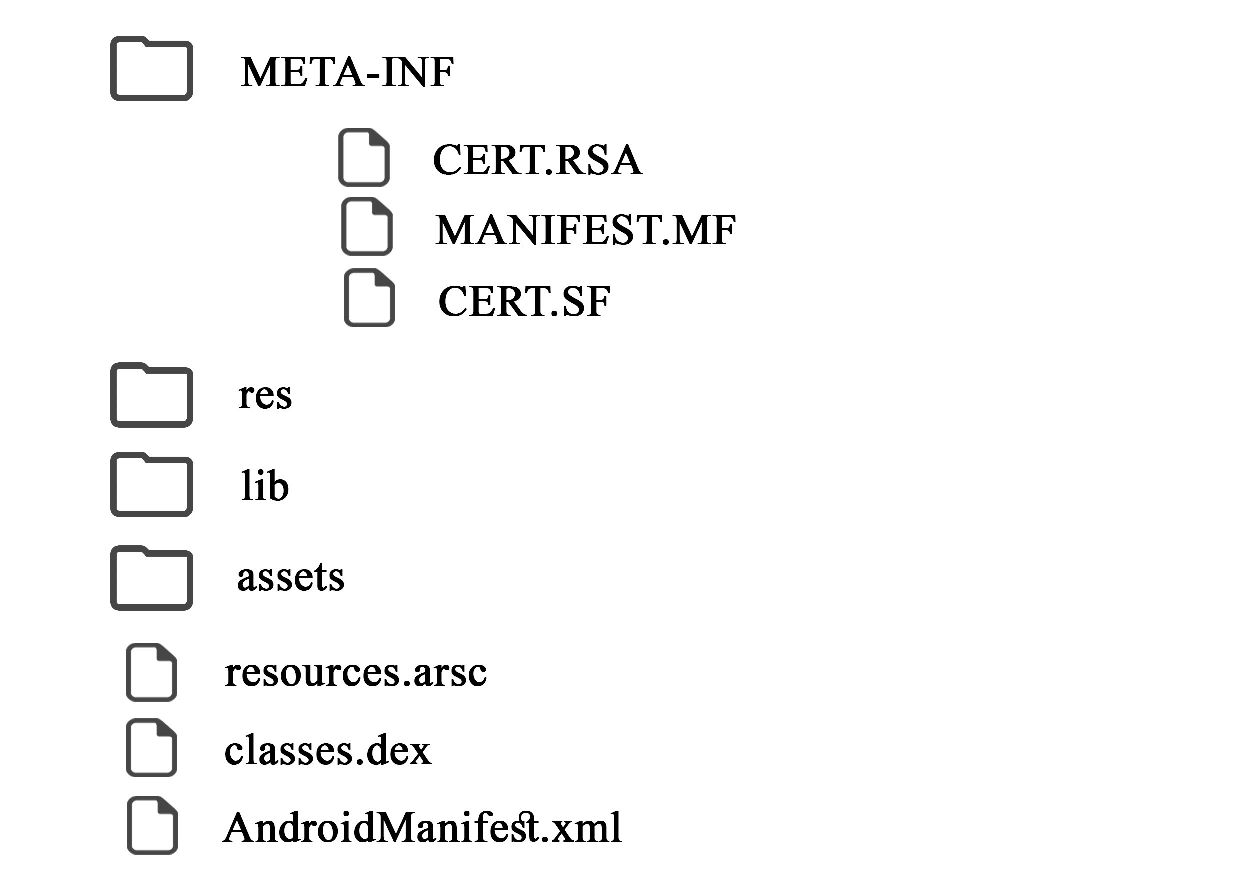
\includegraphics[width=60mm]{images/apkStructure.pdf}
  \end{center}
  \caption{Typická štruktúra APK súboru}
  \label{fig:strukturaApk}
\end{figure}


V~APK súbore nájdeme nasledujúce súbory a adresáre:
\begin{itemize}

	\item \bod{AndroidManifest.xml} -- súbor obsahujúci meta informácie o~aplikácii. Pomocou tohto súboru oznamuje aplikácia operačnému systému svoju identitu a požiadavky. Android Manifest sa v~APK balíčku nachádza vo formáte skompilovaného binárneho XML.
Súbor AndroidManifest.xml obsahuje okrem iného informácie o~nasledujúcich vlastnostiach aplikácie:
		
		\begin{itemize}
			\item meno balíka aplikácie slúžiace ako unikátny identifikátor aplikácie,
			\item najnižšiu verziu Android API na ktorej je aplikácia spustiteľná,
			\item popisuje základné komponenty aplikácie, obsahuje informácie o~aktivitách, službách (service), poskytovateľoch obsahu (content provider), prijímačoch (broadcast receiver) a triedach, ktoré ich v~rámci aplikácie implementujú,
			\item deklaruje povolenia vyžadované aplikáciou na prístup k~zabezpečeným častiam Android API,
			\item definuje povolenia vyžadované od iných aplikácií pri interakcii s~danou aplikáciou~\cite{Manifest}.
		\end{itemize}
	
	\item \bod{Classes.dex} -- súbor obsahujúci spustiteľný kód aplikácie. Súbor typu DEX (Dalvik Executable) obsahuje operačné kódy a inštrukcie špecifické pre behové prostredie Android Runtime a virtuálny stroj Dalvik Virtual Machine (pre verzie Android 4.4.4 a staršie)~\cite{DexFormat}. 

	\item \bod{Resources.arsc} -- obsahuje informácie o~zdrojových súboroch aplikácie. Tento súbor určuje vzťah medzi zdrojovými súbormi a ich identifikátormi, pomocou ktorých sú súbory referencované v~zdrojovom kóde aplikácie.
	
	\item \bod{Assets} -- adresár obsahujúci neskomprimované zdrojové súbory.  Na rozdiel od zdrojových súborov z~priečinku res, tieto zdroje nie sú referencované identifikátorom, ale prístup k~nim je umožnený pomocou API triedy \zv{AssetManager}.
	
	\item \bod{Lib} -- v~tomto adresári sa nachádzajú skompilované knižnice určené pre konkrétnu architektúru procesora. Medzi podporované architektúry patrí ARMv7 a novšie, x86, x86\_64.

	\item \bod{Res} -- adresár obsahujúci zdroje aplikácie. Obsah tohto adresára je tvorený predovšetkým multimediálnymi súbormi ako napríklad obrázky a ikony, ale aj súbormi vo formáte XML ktoré definujú užívateľské rozhranie, farby, lokalizované texty alebo štýl aplikácie. Súbory umiestnené v~tomto adresári sú v~zdrojovom kóde referencované pomocou unikátnych číselných identifikátorov, ktoré sú vygenerované počas kompilácie a nachádzajú sa v~triede \zv{R.java}. Obsah priečinku je ďalej logicky členený do viacerých podpriečinkov. Android podporuje lokalizáciu a rôzne verzie zdrojových súborov, ktoré použije na základe údajov o~zariadení na ktorom je aplikácia spustená~\cite{Resources}.
	
	\item \bod{META-INF} -- v~tomto adresári sa nachádzajú súbory zaručujúce digitálny podpis a integritu APK balíčka. 
		\begin{itemize}
			\item CERT.RSA  -- súbor obsahujúci certifikát podpisu aplikácie.
			\item MANIFEST.MF  -- súbor obsahujúci hash každého súboru v~APK archíve. Využíva hashovaciu funkciu \zv{SHA-1}.
			\item CERT.SF  -- súbor obsahujúci záznam o~každom súbore v~APK archíve. Záznam o~jednom súbore obsahuje jeho názov a \zv{SHA-1} hash záznamu o~tomto súbore z~MANIFEST.MF.
		\end{itemize}		
		
		
\end{itemize} 


\section{Distribúcia aplikácií}
Aplikácie na platforme Android sú distribuované ako inštalačné APK balíčky. 
Podľa formy distribúcie a inštalácie môžeme aplikácie rozdeliť na dve základné skupiny:
\begin{itemize}
 \item \bod{Predinštalované (systémové) aplikácie} -- tieto aplikácie sú distribuované priamo so systémom a sú nainštalované pri iniciálnom spustení systému,
 \item \bod{Užívateľské aplikácie} -- aplikácie distribuované vo forme balíčkov poskytovaných najčastejšie pomocou obchodov s~aplikáciami.
\end{itemize}

Zoznam predinštalovaných aplikácií určuje výrobca zariadenia. Používateľ nemá možnosť systémové aplikácie odinštalovať. Do kategórie predinštalovaných systémových aplikácií patria aplikácie umožňujúce ovládanie základného vybavenia zariadenia ako napríklad aplikácia telefón alebo fotoaparát. Do tejto kategórie patria aj predinštalované služby od spoločnosti Google. 

Užívateľské aplikácie slúžia na prispôsobenie systému pre potreby konkrétneho užívateľa. O~inštalácii a odstránení užívateľských aplikácií rozhoduje používateľ. Na pohodlné prehliadanie a inštaláciu aplikácií slúžia obchody (app stores). Pomocou centralizovaných obchodov s~aplikáciami môžu softvéroví vývojári jednoducho distribuovať svoju aplikáciu k~veľkému počtu užívateľov.  Najrozšírenejším a najznámejším obchodom s~aplikáciami pre platformu Android je oficiálny obchod \zv{Google Play Store}. 

Okrem oficiálneho obchodu sú aplikácie distribuované aj pomocou alternatívnych distribučných kanálov. Medzi takéto kanály zaraďujeme alternatívne obchody s~aplikáciami ako napríklad \zv{Amazon Appstore}. Častým distribučným kanálom sú aj obchody výrobcov mobilných zariadení alebo obchody mobilných operátorov. Existuje viacero služieb tretích strán, ktoré sprostredkovávajú prístup k~oficiálnym aplikáciám z~týchto obchodov. APK súbory sú distribuované aj pomocou warezových portálov na zdieľanie súborov alebo underground obchodov. 

Z~dôvodu udržania bezpečného a spoľahlivého fungovania platformy Android je dôležitá bezpečnosť a kvalita distribuovaných aplikácií. Výskum porovnávajúci kvalitu aplikácií na neoficiálnych distribučných platformách ukázal, že tieto distribučné kanály obsahujú $5$ až $13\%$ aplikácií, ktoré sú klonom oficiálnych aplikácií distribuovaných pomocou \zv{Google Play Store}~\cite{Zhou2012}.

\section{Inštalácia aplikácií}

Platforma Android poskytuje služby na inštaláciu, aktualizáciu a odinštalovanie aplikácií. \newline
Základnú funkcionalitu poskytujú nasledujúce služby.
\begin{itemize}
	\item \bod{Package Installer} -- implementuje funkcionalitu inštalácie, aktualizácie a odinštalovania aplikácií,
	\item \bod{Package Manager Service} -- poskytuje API pre správu nainštalovaných softvérových balíčkov,
	\item \bod{Daemon Installd} -- vytvára a spravuje adresáre potrebné pre nainštalovanie aplikácie.
\end{itemize}
Inštalácia aplikácie pozostáva z~overenia aplikácie a extrakcie dát z~APK balíčka. Aplikácia je overená na základe digitálneho podpisu a metadát zo súboru \zv{AndroidManifest.xml}. Systémové aplikácie sú rozbalené do adresára \cesta{/system/app}. Užívateľské aplikácie sú nainštalované v~adresári \cesta{/data/app}. Systém Android uchováva v~spomínaných adresároch kompletné APK súbory~\cite{AndroidDeveloper,Hashimi2009}.

\section{Bezpečnosť}

Bezpečnosť a integrita distribuovaných APK balíčkov je dôležitým aspektom zabezpečenia celého systému Android.

\subsection{Podpis aplikácie}

Každý APK balíček musí byť digitálne podpísaný. Systém Android zabráni inštalácii digitálne nepodpísaných aplikácií. 
Súbory súvisiace s~podpisom APK balíčka sa nachádzajú v~priečinku \zv{META-INF}. Počas digitálneho podpisu aplikačného balíčka sa vygenerujú \zv{SHA-1} alebo \zv{SHA-256} hashe súborov obsiahnutých v~APK archíve. Záznamy o~súboroch a ich hashoch sú uložené v~súboroch \cesta{META-INF/MANIFEST.MF} a \cesta{META-INF/CERT.SF}. Celý APK balíček je následne podpísaný pomocou utility \zv{Jarsigner}. 

Android podporuje dve schémy digitálneho podpisu aplikácie. Schéma verzie 1 je založená na podpise štandardného Java balíčka. Táto schéma nechráni niektoré súbory nachádzajúce sa v~APK balíčku, ako napríklad metadáta o~ZIP archíve. Počas procesu overenia APK balíčka podpísaného touto schémou je potrebné rozbaliť súbory obsiahnuté v~archíve. Po rozbalení celého balíčka sú nepodpísané súbory odstránené. Nutnosť rozbaliť a sprocesovať všetky súbory bez ich predchádzajúceho overenia predstavuje výrazné bezpečnostné riziko. Potreba dekomprimovania súborov počas procesu overenia APK balíčka výrazne zvyšuje časovú a pamäťovú náročnosť tejto operácie.  Od verzie Android 7.0 (verzia API 24) je podporovaná schéma podpisu vo verzii 2, ktorá je špecializovaná na podpis APK balíčka a eliminuje nedostatky predchádzajúcej verzie. V~súčasnosti sú aplikácie zvyčajne podpísané obidvomi spôsobmi čo zvyšuje ich kompatibilitu s~rôznymi verziami systému. Aplikácie podpísané pomocou schémy podpisu verzie 2 sú na systémoch Android 7.0 a novších nainštalované rýchlejšie a bezpečnejšie. Schéma podpisu nie je spätne kompatibilná a staršie verzie operačného systému vyžadujú aplikácie podpísané verziou 1~\cite{NT0FrzQIkOAYbG2Ga}.

\subsubsection{\textbf{Kontrola integrity}}
Počas digitálneho podpisu sú vygenerované hashe súborov z~APK balíčka. Tieto hashe slúžia na zaručenie integrity. Počas inštalácie aplikácie sa v~rámci procesu overenia aplikácie kontrolujú hashe jednotlivých súborov. V~prípade zmeny súborov v~aplikácii bez jej opätovného podpisu systém zabráni inštalácii. Pri zmene obsahu musí byť APK balíček podpísaný znova. 

\subsubsection{\textbf{Identifikácia autora}}
Podpis balíčka slúži na identifikáciu autora aplikácie. V~prípade, že je viacero aplikácií podpísaných jedným kľúčom, pochádzajú tieto aplikácie od jedného vydavateľa. 
Všetky verzie jednej aplikácie musia byť podpísané rovnakým certifikátom. Unikátnym identifikátorom aplikácie je meno hlavného balíka aplikácie (package name). Android považuje aplikácie s~rovnakým menom balíka za rôzne verzie jednej aplikácie a pri aktualizácii nahrádza staršiu verzie novšou. Všetky aplikácie s~rovnakým menom balíka musia byť preto podpísané rovnakým privátnym kľúčom, čo zaručuje, že pochádzajú od rovnakého vydavateľa.  V~prípade, že sú podpísané rôznymi kľúčmi, Android ich inštaláciu zamietne. 

\subsubsection{\textbf{Správa podpisových kľúčov}}
Platforma Android povoľuje používanie tzv. \zv{self-signed} certifikátov. \zv{Self-signed} certifikáty sú podpísané identitou, ktorú identifikujú. 

Z~pohľadu vývojára je správa podpisového kľúča veľmi dôležitá. Vývojári aplikácií majú pri správe podpisového kľúča dve možnosti. Môžu používať manuálnu správu, alebo službu \zv{Google Play App Signing}. 
\begin{itemize}
	\item \bod{Manuálna správa kľúča} -- v~prípade použitia manuálnej správy kľúča je aplikácia podpísaná vývojárom a nahraná do obchodu s~aplikáciami. Odtiaľ je ďalej distribuovaná k~užívateľom. V~prípade straty podpisového kľúča nie je vývojár aplikácie schopný vydávať nové verzie aplikácie pod rovnakým názvom balíka.
	\item \bod{Google Play App Signing} -- pri použití bezpečnej správy podpisových kľúčov \zv{Google Play App Signing} je kľúč používaný na podpis balíčka spravovaný službou  \zv{Google Play}. Vývojár podpíše aplikáciu svojim kľúčom používaným na komunikáciu so službou  \zv{Google Play}. Po nahratí na \zv{Google Play} je balíček nanovo podpísaný podpisovým kľúčom. Aplikácia distribuovaná k~užívateľom je teda podpísaná kľúčom manažovaným službou \zv{Google Play}~\cite{NT0FrzQIkOAYbG2G}. 
\end{itemize}


\subsection{Známe bezpečnostné riziká}

Existuje viacero známych zraniteľností súvisiacich s~distribúciou aplikácií  pre platformu Android. Najviac rozšíreným problémom je prebaľovanie APK balíčkov. Pri tomto procese je aplikácia rozbalená a niektoré časti aplikácie sú upravené. Detailný popis prebaľovania aplikácií a rizík s~tým spojených sa nachádza v~kapitole \ref{chap:repackaging}.

Metóda prebaľovania upraví aplikáciu a nanovo ju podpíše iným podpisovým kľúčom. Ďalšie známe metódy útokov využívajú predovšetkým zraniteľnosti pri overovacom procese APK balíčka a nemodifikujú originálny podpis. 

Zraniteľnosť pri inštalácií nekompletného APK súboru využíva fakt, že pri overovaní hashov súborov sa ignorujú záznamy, ktoré v~balíku neexistujú. Súbory je teda možné z~APK archívu odstrániť bez jeho opätovného podpísania. Modifikovanú aplikáciu je možné distribuovať ako originálnu verziu. Aplikácia po odstránení súborov nebude pracovať správne a môže dostať celé zariadenie do nepoužiteľného stavu. Tento útok patrí do kategórie \zv{denial of service}~\cite{A7idcou1z6WqKvQZ}.

Pri verifikačnom procese sa nekontrolujú súbory slúžiace na podpis balíčka. To umožňuje útočníkovi nahrať do adresára \zv{META-INF} ľubovoľný súbor bez potreby opätovného podpísania. Útočník tak môže do tohto adresára nahrať časti skompilovaného zdrojového kódu. Tento kód však nevykoná pôvodná aplikácia, ktorej zdrojové kódy zostali nepozmenené. Takýto škodlivý obsah môže byť dlhodobo neaktívny. Za účelom vykonania tohto kódu musí utočník distribuovať vlastnú aplikáciu, ktorá skúma inštalačné archívy všetkých nainštalovaných aplikácií a hľadá v~nich vložené škodlivé časti. V~prípade, že ich nájde, načíta tieto predpripravené časti implementujúce škodlivé správanie a použije ich. Pomocou tohto spôsobu je možné efektívne zabrániť detekcií škodlivého správania antivírusovými programami, pretože jednotlivé inštrukcie môžu byť ditribuované pomocou viacerých aplikačných archívov~\cite{A7idcou1z6WqKvQZ}.
